\chapter{Implementierung}
\label{chap:Implementierung}

Die Anwendung RoCoVoMo wird in der Programmiersprache Java geschrieben und verwendet diverse Frameworks, die im folgenden kurz beschrieben werden:

\begin{itemize}
\item \textit{\gls{OSGi}}: Erm\"oglicht die Aufteilung der einzelnen Komponenten der Anwendung in sogenannte \textit{Bundles} oder Module die getrennt voneinander verwendet werden k\"onnen
\item \textit{jahmm}: Liefert alle Algorithmen und Komponenten, die zur Erstellung von \glspl{HMM} ben\"otigt werden
\item \textit{jnect}: Dient als Schnittstelle zwischen Kinect, Kinect SDK for Windows und der Java-Anwendung
\item \textit{lwjgl}: Erm\"oglicht die Verwendung von drei dimensionalen Grafiken der OpenGL Bibliothek
\end{itemize}

Dar\"uber hinaus wird die gesamte Java-Anwendung innerhalb der \gls{Eclipse} \gls{IDE} entwickelt und auf der aktuellen Juno 4.2 Plattform umgesetzt. Die Anwendung selbst wird in Form einer \gls{RCP} entwickelt und damit das \gls{OSGi} Framework von Eclipse, \gls{Equinox}, verwendet.
\newline
Im Folgenden werden die einzelnen Bestandteile der Anwendung n\"aher beschrieben.

\section{Architektur --- Design}
Seit den Arbeiten an der Anwendung f\"ur den ersten Teil der Arbeit wurde das Design und die Architektur der Anwendung nochmals \"uberarbeitet. Abbildung~\ref{fig:architecture} zeigt den aktuellen Stand der Anwendung.
\newline
Die Arbeiten an der Architektur entfielen auf beide Autoren gleicherma\ss en, wobei Volker Werling einen Gro\ss teil der \"Uberarbeitung des Designs f\"ur den zweiten Teil der Studienarbeit \"ubernahm.

\begin{figure}[htb]
\centering
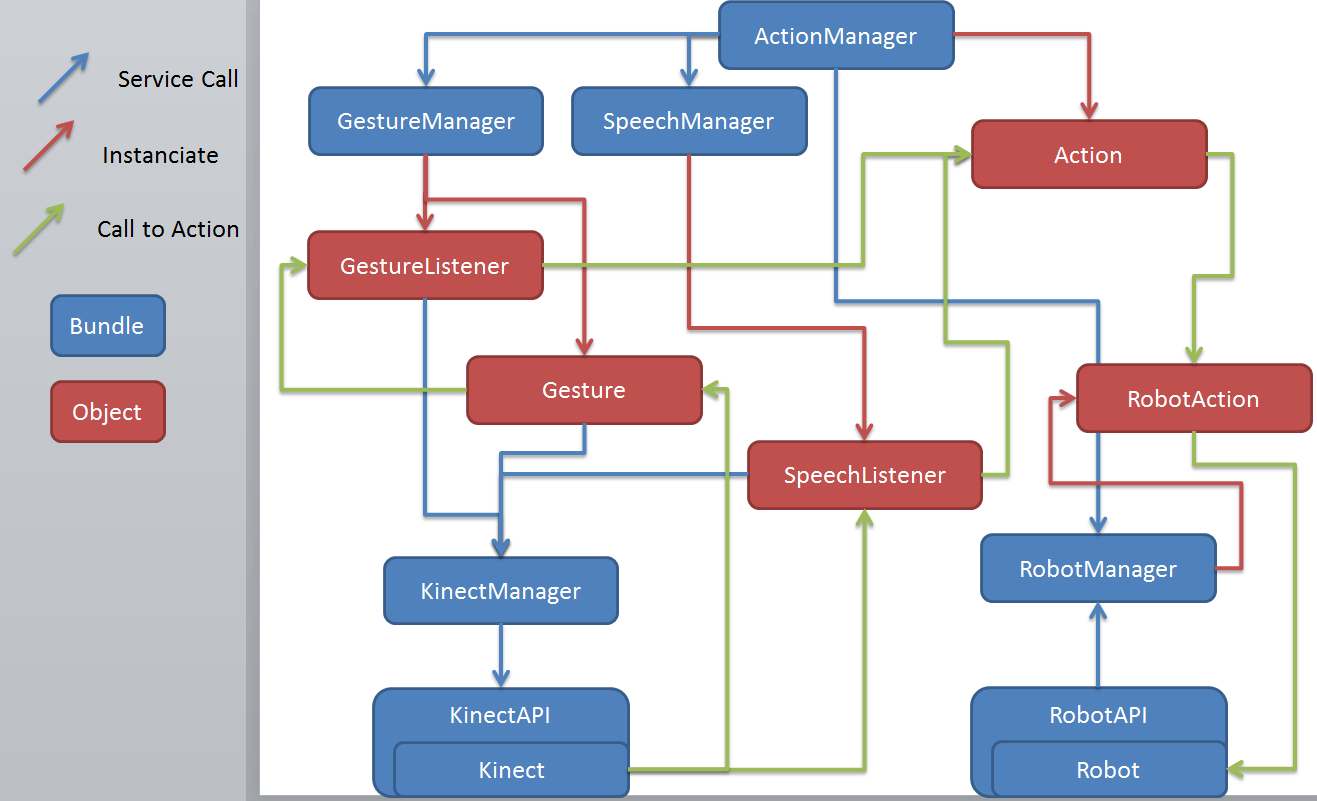
\includegraphics[width=0.8\textwidth]{img/impl/architecture.png}
\caption[Architekturdiagramm der Anwendung RoCoVoMo]{Architekturdiagramm der Anwendung RoCoVoMo}
\label{fig:architecture}
\end{figure}

Die mit der Farbe Blau markierten Elemente stellen sogenannte \gls{OSGi}-Bundles dar. Dabei handelt es sich vereinfacht gesprochen um einen Container, der eine bestimmte Logik beziehungsweise Fachlichkeit abdeckt und modular verwendbar ist. In der Anwendung RoCoVoMo werden mehrere solcher Bundles verwendet, die im Folgenden weiter beschrieben werden. Mit Rot markierte Elemente sind Java Klassen, die als Objekte innerhalb der Bundles verwendet werden.

\subsection{ActionManager}
In einer sogenannten \textit{Managerklasse}, in diesem Fall dem \textit{ActionManager} werden alle Aktionen verwaltet, die innerhalb der Anwendung ausf\"uhrbar sind. Die Managerklasse f\"uhrt dabei selbst keine Fachlichkeit aus, sondern delegiert diese an die darin verwalteten Objektinstanzen weiter, hier den einzelen Aktionen und ebenso an damit verbundene Bundles, hier \textit{GestureManager}, \textit{SpeechManager} und \textit{RobotManager}.
\newline
Diese Aufteilung erm\"oglicht es, Aktionen flexibel in die Anwendung zu integrieren, abzu\"andern oder gar zu l\"oschen. Weiter ist durch die loose Verbindung \"uber sogenannte \textit{Service Calls}, zum Beispiel des GestureManagers keine Abh\"angigkeit zu darin verwalteten Gesten vorhanden. Die einzige Verbindung zwischen Gesten und Aktionen findet im GestureListener statt, hierzu sp\"ater mehr.
\newline
Gleiches gilt f\"ur Sprache und der Roboteransteuerung.

\subsubsection{Action}
Die \textit{Action} ist so konzipiert, dass sie nicht direkt von einem Robotertyp abh\"angig ist. Diese Design erm\"oglicht sogar den relativ einfachen Umbau der Anwendung und Einsatz eines alternativen Robotermodells zum Lego NXT.
\newline
Wird eine Aktion ausgef\"uhrt, so ruft diese weiter die \textit{RoboterAction} aus, die die weitere Steuerung des Roboters \"ubernimmt, bisher der Lego NXT. Aufgerufen wird dieses Objekt von den Objekten \textit{GestureListener}, und \textit{Speechlistener}.

\subsection{GestureManager}
\textit{GestureManager} verwaltet alle in der Anwendung verf\"ugbaren Gesten. Dabei existiert pro \textit{Gesture}-Objekt ein \textit{GestureListener}.

\subsubsection{GestureListener}
\textit{GestureListener} liest Kinectinformationen aus und gleicht diese mit den \glspl{HMM} ab. Dabei werden \"uber spiezelle \textit{Recognizer}-Klassen, die Kinectdaten als HMM-Sequenzen eingelesen und Wahrscheinlichkeitsauswertungen im \gls{HMM} die richtige Geste erkannt und das entsprechende \textit{Gesture}-Objekt in Folge ausgef\"uhrt.

\subsubsection{Gesture}
\textit{Gesture} beinhaltet zahlreiche Meta-Informationen \"uber die entsprechende Geste und ist \"uber einen \textit{Actioncall} mit dem zugewiesenen \textit{Action}-Objekt verbunden. Wird das Gesture-Objekt vom Listener ausgef\"uhrt, so ruft Gesture diese Aktion auf.

\subsection{SpeechManager}
\textit{SpeechManager} verwaltet alle Sprachbefehle. Da Sprachbefehle bereits innerhalb der Kinect SDK integriert sind, und dieser lediglich \"uber String-Objekte und der entsprechenden Sprache hinzugef\"ugt werden m\"ussen, wurde darauf verzichtet ein gesondertes Objekt {Speech} zu modellieren, da dieses ledigliche die String Information enthalten w\"urde. Diese Daten sind im \textit{SpeechListener} hinerlegt.

\subsubsection{SpeechListener}
\textit{SpeechListener} f\"uhrt, sobald ein Sprachbefehl von der Kinect erkannt wurde, das entsprechende \textit{Action}-Objekt aus.

\subsection{KinectManager}
\textit{KinectManager} verwaltet die Verwendung von und den Datenaustausch mit der Kinect. Dieser wird von den Objekten \textit{GestureListener}, \textit{Gesture}, und \textit{SpeechListener} \"uber Service Calls aufgerufen.
\newline
Durch den Manager wird die KinectAPI und darin enthaltene Kinect f\"ur alle Teilnehmer sichtbar und dadurch kann ohne direkte Abh\"angigkeiten auf die Kinectinformationen zugegriffen werden.

\subsection{RobotManager}
\textit{RobotManager} verwaltet die Verwendung der RobotAPI und des darin enthaltenen Roboters. Bisher wird dadurch der Lego NXT verbunden. Durch diese Architektur ist jedoch auch m\"oglich weitere Robotermodelle in die Anwendung RoCoVoMo zu integrieren und weitere Abh\"angigkeiten zu erhalten.
\newline
Der Manager verwaltet weiterhin die Objekte \textit{RobotAction}, die dann aber je nach Robotermodell individuell geschrieben werden m\"ussen, da diese direkt auf die Roboter \gls{API} zugreifen, und diese sich von Modell zu Modell unterscheiden kann.

\section{Trainingsmodul}
Das Trainingsmodul wurde konzeptionell bereits in Kapitel~\ref{chap:Konzept} beschrieben. In diesem Abschnitt werden die technischen Details dieser Komponente n\"aher erl\"autert.
\newline
Abbildung~\ref{fig:recorder} zeigt einen Ausschnitt des Moduls in der laufenden Anwendung, welche auf einer \gls{RCP} basiert.
\newline
Um Trainingsdaten zu speichern muss zu Beginn eine Geste ausgew\"ahlt werden, und anschlie\ss end der Intervall Parameter angegeben werden, nach wie viel Sekunden die Elementkoordinaten der Kinect gespeichert werden sollen. Sofern eine Datei zum Speichern der Werte ausgew\"alt wurde, kann \"uber Start die Aufzeichnung beginnen. In der linken H\"alfte des Fensters werden anschlie\ss end die Werte angezeigt und \"uber den Button Preview kann dar\"uber hinaus der derzeitige Inhalt der Datei betrachtet werden, was f\"ur Experten eine Erleichterung bei Fehlersuche oder Korrekturen darstellt.
\newline
Dieser Vorgang wurde simpel konzipiert und es ist nicht schwer, sich in der Anzeige zurecht zu finden, jedoch erfordert das Aufzeichnen der Daten einiges an Training und Geduld, und muss mit Sorgfalt geschehen, da die nur mit korrekten und sauberen Trainingsdaten eine effektive Gestensteuerung erm\"oglicht werden kann. Dar\"uber hinaus muss dieser Vorgang vielfach wiederholt werden, da nur \"uber eine Vielzahl von Trainingsdaten ein stabiles \gls{HMM} generiert werden kann. Als Richtwert sollten stets zwischen 80 und 100 Sequenzen in einem Trainingssatz f\"ur eine Geste vorhanden sein.
\newline
Die Arbeiten an diesem Modul wurden von Simon Ebner durchgef\"uhrt.

\section{Kinect-Modul}
Das Konzept des Kinect-Moduls wurde bereits in Kapitel~\ref{chap:Konzept} erl\"autert. Hier wird weiter auf die technischen Feinheiten dieser Komponente eingegangen.
\newline
Ein Aussschnitt des Moduls inst in Abbildung~\ref{fig:view} dargestellt. Dieser zeigt die grafische Darstellung eines sogenannten \textit{Skeletons} der Kinect, innerhalb der Anwendung RoCoVoMo.
\newline
Ein Gro\ss teil der Informationen die f\"ur die Darstellung dieses grafischen Objekts notwendig sind, liefert das \textit{jahmm}-Framework. In der Anwendung RoCoVoMo werden diese Daten \"uber das KinectManager Bundle bereitgestellt und k\"onnen so in einem sogenannten \textit{View} angezeigt werden. Diese Anzeige kann auch w\"ahrend der Trainingsaufzeichnung, oder der Robotersteuerung  weiterlaufen und beeinflusst nicht die Performance der Anwendung.
\newline
Sobald das Modul gestartet wird, verbindet sich das View automatisch mit der Kinect Instanz und die grafische Anzeige wird generiert.
\newline
Die Arbeiten an diesem Modul wurden von Simon Ebner durchgef\"uhrt.

\section{Roboterinterface}
Das Roboterinterface wurde konzeptionell bereits in Kapitel~\ref{chap:Konzept} beschrieben. In diesem Abschnitt werden die technischen Details dieser Komponente n\"aher erl\"autert. Dabei muss jedoch angemerkt werden, dass die Umsetzung dieses Moduls in Form eines \gls{GUI} aus Zeitgr\"unden nicht m\"oglich war. Die Arbeiten an diesem Modul wurden aufgrund des Umfangs auf beide Autoren verteilt. Volker Werling arbeitete an der Robotersteuerung und den Sprachbefehlen, und Simon Ebner an den Bereichen \gls{HMM}, sowie Design und Gestaltung der Gesten.
\newline
Ziel der Arbeiten an diesem Modul war es ein drei dimensionales grafisches Interface zu gestalten, in dem der User eine vereinfachte Sicht der Roboters, sowie eine Anzeige seiner Eingaben, wie Gesten und Sprachbefehle, und eine Ausgabe der jeweilgen erkannten Aktion. Als Zeitraubend hat sich dabei die Kombination und Interkation der vielen Komponenten dieses Interfaces erwiesen. So konnten ohne Trainingsdaten nur Simulationen durchgef\"uhrt werden und die Robotersteuerung war auf einzelne vordefinierte sequenzielle Anweisungen beschr\"ankt. Weiterhin stellte sich die Erstellung des grafischen Interfaces an sich als Herausforderung heraus, in dem Sinne, dass die Autoren bislang nur wenig Erfahrung mit 3D Design und Entwicklung von OpenGL Anwendungen hatten.

\begin{figure}[htb]
\centering
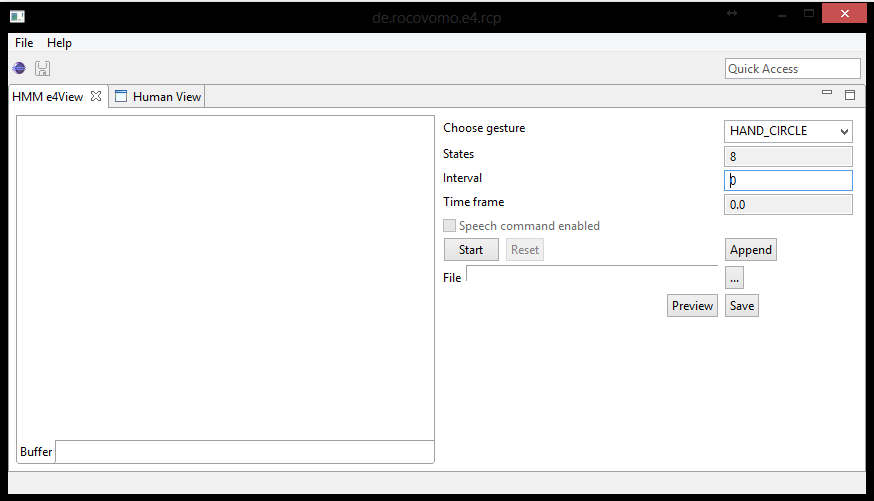
\includegraphics[width=0.8\textwidth]{img/impl/recorder.png}
\caption[Ausschnitt des Trainingsmoduls der RoCoVoMo Anwendung]{Ausschnitt des Trainingsmoduls der RoCoVoMo Anwendung}
\label{fig:recorder}
\end{figure}

\begin{figure}[htb]
\centering
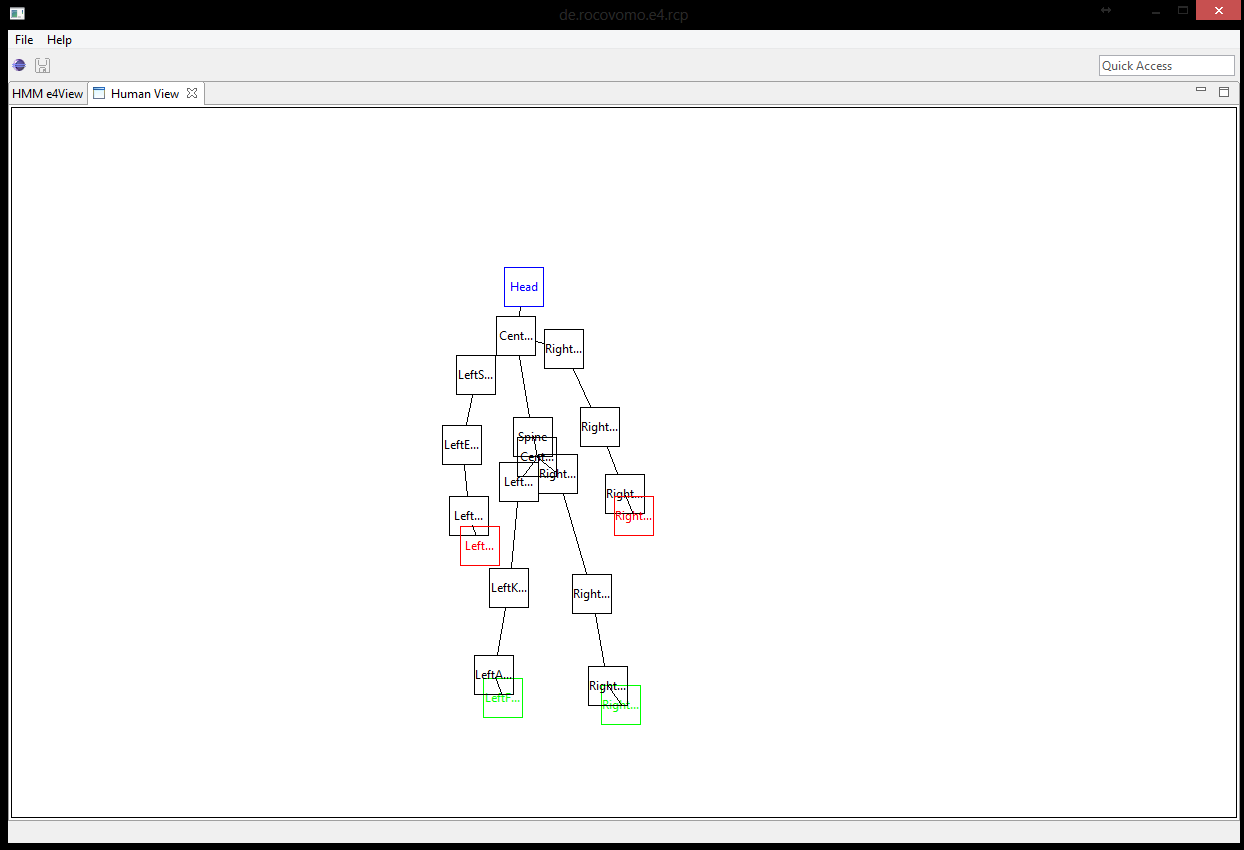
\includegraphics[width=0.8\textwidth]{img/impl/humanview.png}
\caption[Ausschnitt des Kinect-Moduls der RoCoVoMo Anwendung]{Ausschnitt des Kinect-Moduls der RoCoVoMo Anwendung}
\label{fig:view}
\end{figure}